\documentclass[10pt]{article}
\usepackage[latin1]{inputenc}
\usepackage{amsmath}
\usepackage{microtype}
\usepackage[none]{hyphenat}
\usepackage{verbatim}
\usepackage{amsfonts}
\usepackage{amssymb}
\usepackage{enumitem}
\renewcommand{\familydefault}{\sfdefault}
\usepackage{mathpazo}
\renewcommand{\rmdefault}{put}
\usepackage{enumitem}
\usepackage[dvipsnames,svgnames]{xcolor}
\usepackage{tkz-euclide}
\usetkzobj{all}
\usepackage{graphicx}
\usetikzlibrary{calc,patterns,angles,quotes}
\usepackage{tikz} 	
\usepackage{adjustbox}
\usepackage{multicol}
\usepackage{lipsum}
\usepackage[left=0.1cm,right=0.7cm,top=0.2cm,bottom=1.5cm,paperheight=15cm,paperwidth=8.5cm]{geometry}
\usepackage{cancel} \usepackage{xcolor}
\usepackage{tcolorbox}
\usetikzlibrary{decorations.pathmorphing,patterns,shapes.geometric}
\usetikzlibrary{decorations.pathreplacing,calc}
 \newcommand\coret[2][red]{\renewcommand\CancelColor{\color{#1}}\cancel{#2}}
\SetLabelAlign{Center}{\hfill\makebox[1.0em]{#1}\hfill}

%%_------= solusi


% Set this =0 to hide, =1 to show

% Set this =0 to hide, =1 to show
\newtcolorbox{mybox}[1][] { colframe = blue!10, colback = blue!3,boxsep=0pt,left=0.2em, coltitle = blue!20!black, title = \textbf{jawab}, #1, } 

%---------- jika kunci muncul =1 -
\def\tampilkunci{1}
\newcommand{\hide}[1]{\ifnum\tampilkunci=1
%
\begin{mybox}
 #1
\end{mybox}
%
\vspace{\baselineskip}\fi}



\newcommand*\cicled[1]{\tikz[baseline=(char.base)]{\node[white, shape=circle, fill=red!80,draw,inner sep=0.5pt](char){#1};}}

\newcommand*\kunci[1]{\ifnum\tampilkunci=1
%
\tikz[baseline=(char.base)]{\node[red, shape=circle,draw,inner sep=0.5pt](char){#1};}
\stepcounter{enumii}%
%
\fi\ifnum\tampilkunci=0
%
\hspace{3pt}#1\stepcounter{enumii}%
\fi}

\newcommand*\silang[1]{\tikz[baseline=(char.base)]{
\draw[red,thick](-0.2,-0.20)--(0.2,0.2);
\draw[red,thick](-0.2,0.20)--(0.2,-0.2);
\node[black](char){#1};
}}


\newcommand*\centang[1]{\tikz[baseline=(char.base)]{
\draw[red, very thick](-0.2,0.1)--(-0.1,0)--(0.2,0.3);
\node(char){#1};
}}

\newcommand*\merah[1]{
\textcolor{red}{#1}}
\newcommand*\pilgan[1]{
\begin{enumerate}[label=\Alph*., itemsep=0pt,topsep=0pt,leftmargin=*, align=Center] #1 
\end{enumerate}}
\newcommand*\pernyataan[1]{
\begin{enumerate}[label=(\arabic*), itemsep=0pt,topsep=0pt,leftmargin=*] #1 
\end{enumerate}}



\begin{document}

\setlength{\abovedisplayskip}{0pt}
\setlength{\belowdisplayskip}{3pt}
\setlength{\abovedisplayshortskip}{0pt}
\setlength{\belowdisplayshortskip}{3pt}
%-----------------------------------------------

 \centering
  \renewcommand{\arraystretch}{2}
  \begin{tabular}{  |>{\centering\arraybackslash}m{4cm}|%
                    >{\centering\arraybackslash}m{11cm}|%
                    >{\centering\arraybackslash}m{4cm}|%
  }
    \hline
    \vspace{0.15cm} 
    \tikz[baseline=(char.base)]{
\draw[green!80!black](-0.3,-0.2) rectangle (0.3,0.2);
\node[green](char){line};
} \small{ arifstwan} &       \textbf{Ujian Nasional Fisika 2017 } 
          & arif.stwan@gmail.com 
  \\ \hline 
    
  \end{tabular}
\setlength{\columnsep}{0.2cm}
\renewcommand{\columnseprulecolor}{\color{blue!40}}

\vspace{0.15cm}

\begin{multicols*} {2} 
 \setlength{\columnseprule}{0.4pt}
\newcommand{\tikzmark}[2]{\tikz[remember picture,baseline=(#1.base)]{\node[inner sep=0pt] (#1) {#2};}} 


\begin{enumerate}[itemsep=0mm]
\renewcommand\arraystretch{1}
%--------- nomor 1 --------------
\item  Besaran-besaran di bawah ini yang merupakan besaran turunan adalah... 
\pilgan{
\item gaya, kecepatan dan \coret{panjang}
\item berat, daya dan \coret{waktu}
\item i\coret{massa}, \coret{waktu} dan percepatan
\item berat, energi, dan \coret{massa}
\item [\kunci{E.}] tekanan, gaya dan berat
}

%-------- nomor 2------------
\item Percepatan adalah kecepatan per satuan waktu. Dimensi percepatan adalah . . . 
\pilgan{
\item M.L.T$^{-2}$
\item M.L.T$^{-1}$
\item [\kunci{C.}]L.T$^{-2}$
\item L.T$^{-1}$
\item L.T
}
\hide{
percepatan adalah kecepatan per satuan waktu
$$ a = \frac{v}{t}=\frac{(m/s)}{(s)}=(m/s^3)= M.T^{-2}$$
}
% ------------ nomor 3 -------
\item Dimensi dari daya adalah. . . . 
\pilgan{
\item M.L.T$^{-2}$
\item M.L.T
\item M.L.T$^{-1}$
\item [\kunci{D.}]M.L$^{2}$T$^{-3}$
\item M.L.T$^{-3}$
}
\hide{
Daya adalah energi per satuan waktu. Salah satu rumus energi yang mudah diingat adalah $E=m.g.h$ dengan $m$ massa (kg), $g$ percepatan gravitasi (m/s$^2$), dah $h$ adalah ketinggian (m)
$$ P=\frac{E}{t}=\frac{m.g.h}{t}=\frac{(kg).(m/s^2).(m)}{s}=M.L^2.T^{-3}$$
}
%----------- nomor 4 -----------
\item Jarak $s$ yang ditempuh sebuah benda sebagai fungsi dari waktu ($t$) dinyatakan $s = \text{A}t^3+\text{B}t^2+\text{C}t$. Dimensi untuk A, B, dan C adalah . . . .
\pilgan{
\item L.T$^{-1}$, L.T$^{-2}$, L.T$^{-3}$
\item L.T$^{-2}$, L.T$^{-1}$, L.T$^{-3}$
\item L.T$^{-3}$, L.T$^{-1}$, L.T$^{-2}$
\item [\kunci{D.}]L.T$^{-3}$, L.T$^{-2}$, L.T$^{-1}$
\item L, L.T, L.T$^{-2}$
}
\hide{
Untuk menentukan dimensi, perlu dketahui bahwa dalam penjumlahan besaran, hanya besaran yang dimensinya sama yang dapat dijumlahkan. Sehingga pada soal tersebut, antara $s$, A.$t^3$ dan B$t^2$ dan C$t$ mempunyai dimensi yang sama.

\begin{align*}s &= \text{A}t^3+\text{B}t^2+\text{C}t\\
\text {L}&=\text{L}+\text{L}+\text{L}
\end{align*}}
\hide{
Sehingga masing-masing suku memiliki dimensi L
\begin{minipage}[t]{0.47\textwidth}
\begin{align*}
\text{A}t^3 &= [L]\\
\text{A}&=\frac{[L]}{t^3}\\
\text{A}&=\frac{[L]}{[T]^3}=L.T^{-3}
\end{align*}
\begin{align*}
\text{B}t^2 &= [L]\\
\text{B}&=\frac{[L]}{t^2}\\
\text{B}&=\frac{[L]}{[T]^2}=L.T^{-2}
\end{align*} \end{minipage}
\begin{minipage}[t]{0.47\textwidth}
\begin{align*}
\text{C}t &= [L]\\
\text{C}&=\frac{[L]}{t}\\
\text{C}&=\frac{[L]}{[T]}=L.T^{-1}
\end{align*}\end{minipage}
}



%---------------- nomor 5 ----------
\item Jika $x$ dalam meter, $t$ dalam sekon, $v$ dalam m/s, dan $a$ dalam m/s$^2$, maka satuan SI dari operasi $\frac{v^2}{x}$ adalah . . . 
\pilgan{
\item [\kunci{A.}] m/s$^2$
\item m/s
\item m$^2$/s$^2$
\item s/m$^2$
\item s$^2$/m
}
\hide{
\begin{align*}
\frac{v^2}{x}&=\frac{(m/s)^2}{m}=\frac{\coret{m}^2.s^{-2}}{m}&= (m.s^{-2})=(m/s^{2})
\end{align*}
}

% ---------------- nomor 6 ------------
\item Hasil penguuran dari jangka sorong pada gambar di bawah adalah . . . .cm 

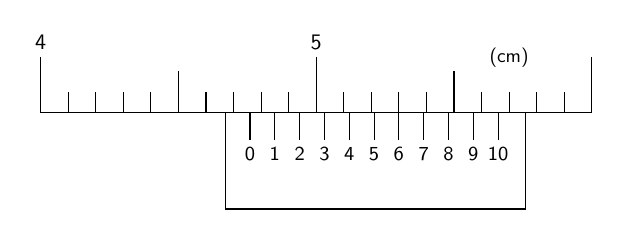
\begin{tikzpicture}[scale=3.5]
\draw[](4,0)--(6,0);
\draw (4.67,0) rectangle (5.76,-0.35);
\node at (5.7,0.2) [scale=0.7]{(cm)};
\foreach \x/\label in {4/4,5/5,6/}{ \draw (\x,0) -- (\x,0.2)node[above,scale=0.8]{\label}; }
\foreach \x in {4.0,4.1,...,6}{ \draw (\x,0) -- (\x,0.075); } \foreach \x in {4.5,5.5}{ \draw (\x,0) -- (\x,0.15); }
\foreach \x [evaluate=\x as \label using \x*0.09+4.76] in {0,1,...,10}
{ \draw (\label ,0) -- (\label ,-0.1)node[below,scale=0.8]{\small{\x}}; 
}
  \end{tikzpicture}

\pilgan{
\item $ 4,86 \pm 0,01$
\item [\kunci{B}]$4,86 \pm 0,005$
\item $4,88 \pm 0,01$
\item $4,88 \pm 0,05$
\item $5,86 \pm 0,005$
}
\hide{
Jangka sorong pada sumbu utama (di kiri angka nol) menunjukkan 4,8 cm. Kemudian angka nonius yang berhimpitan adalah 6. jadi hasil ukurnya adalah. 4,8 + \merah{0,01}$\times$6(cm)=4,86 cm.

Untuk ketidakpastian / ralat pengukuran tunggal menggunakan $\frac{1}{2}$ nilai skala terkecil. Karena nilai skala terkecil jangka sorong adalah \merah{0,01 cm} maka nilai $\frac{1}{2}$NST adalah 0,005 cm. Sehingga hasil ukurnya adalah $$4,86 \pm 0,005 \text{ cm}$$
}
%----------------- nomor 7 -----------
\vspace{1cm}
\item Hasil pembacaan mikrometer skrup di bawah ini adalah . . .mm

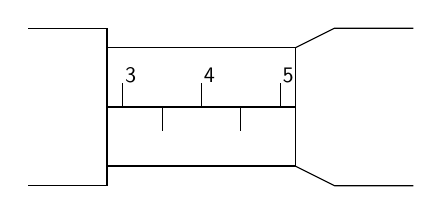
\begin{tikzpicture}
\draw(-1,-1)--(0,-1)--(0,1)--(-1,1);
\draw(0,-0.75) rectangle(2.39,0.75);
\draw (0,0)--(2.39,0);
\draw(2.39,0.75)--(2.89,1)--(3.89,1)(2.39,-0.75)--(2.89,-1)--(3.89,-1);
\foreach \x/\label in {0.2/3,1.2/4,2.2/5} {
\draw (\x,0)--(\x,0.3);
\node at ($(\x,0)+(0.1,0.4)$) [scale=0.8]{\label};
}
\foreach \xb in {0.7,1.7}{
\draw (\xb,0)--(\xb,-0.3);
}



\end{tikzpicture}


\pilgan{
\item $ 4,19 \pm 0,05$
\item $4,20 \pm 0,05$
\item $4,29 \pm 0,005$
\item [\kunci{D.}] $5,19 \pm 0,005$
\item $5,90 \pm 0,01 $
}

%-------------- nomor 8 --------
\item Notasi ilmiah dari bilangan 0,000000022348 adalah . . .. 
\pilgan{
\item $22,348 \times 10^{-9}$
\item $22,348 \times 10^{-10}$
\item $2,23 \times 10^{-8}$
\item [\kunci{D.}]$2,2348 \times 10^{-8}$
\item $2,2348 \times 10^{-9}$
}
\hide{
Penulisan notasi ilmiah yang tepat adalah $2,2348 \times 10^{-8}$. Adapun jika dibulatkan menjadi 3 angka penting menjadi $2,24 \times 10^{-8}$. Sehingga pilihan yang paling tepat adalah \textbf{D}}

%--------------- nomor 9 ---------------
\item Bulatkan angka 0,000849 dalam dua angka penting!
\pilgan {
\item[\kunci{A.}] 0,00085
\item 0,0008
\item 0,0009
\item 0,001
\item 0,00
}
\hide{
Angka 0,000\merah{849} mempunyai tiga angka penting. Untuk membuat menjadi 2 angka penting hanya tinggal dilakukan pembulatan. Hasilnya adalah 0,00085}

%--------------- nomor 10 --------------
\item Hasil pengukuran plat seng menunjukkan panjang 1,50 m dan lebar 1,20 m. Luas plat tersebut menurut aturan angka penting adalah . . . .m$^2$.
\pilgan{
\item 1,8012
\item 1,801
\item 1,81
\item 1,80
\item 1,8
}
\hide{
\begin{tabular}{cc}
1,50 & \\
1,20 & $\times$\\ \hline
1,8000& 
\end{tabular}


}

%------------------ nomor 11 --------
\item Besaran-besaran di bawah ini yang termasuk ke dalam besaran vektor, adalah . . .
\pilgan{
\item tinggi, massa, kecepatan
\item periode, massa, lebar
\item gaya, berat , waktu
\item kecepatan, volume, berat
\item [\kunci{E.}] gaya, kecepatan, berat
}

%---------- nomor 12 ------------
\item Diagram vektor berikut yang menunjukkan \textbf{C=A-B} adalah. . . 


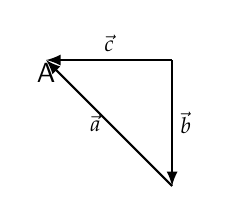
\begin{tikzpicture}[scale=0.8]
%----------------gambar a----------
\node at (-2,-0.2){A};
\draw [thick, -latex](0,0)--node[midway,above,scale=0.8]{$\vec{c}$}(-2,0)coordinate(a);
\draw[thick, -latex](0,0)--node[midway,right,scale=0.8]{$\vec{b}$}(0,-2)coordinate(b);
\draw[thick, -latex](b)--node[midway,left,scale=0.8]{$\vec{a}$}(a);
\end{tikzpicture}
%----------------gambar b----------
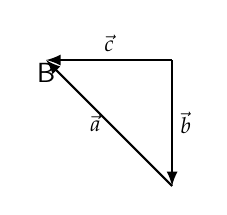
\begin{tikzpicture}[scale=0.8]
\node at (-2,-0.2){B};
\draw [thick, -latex](0,0)--node[midway,above,scale=0.8]{$\vec{c}$}(-2,0)coordinate(a);
\draw[thick, -latex](0,0)--node[midway,right,scale=0.8]{$\vec{b}$}(0,-2)coordinate(b);
\draw[thick, -latex](b)--node[midway,left,scale=0.8]{$\vec{a}$}(a);
\end{tikzpicture}
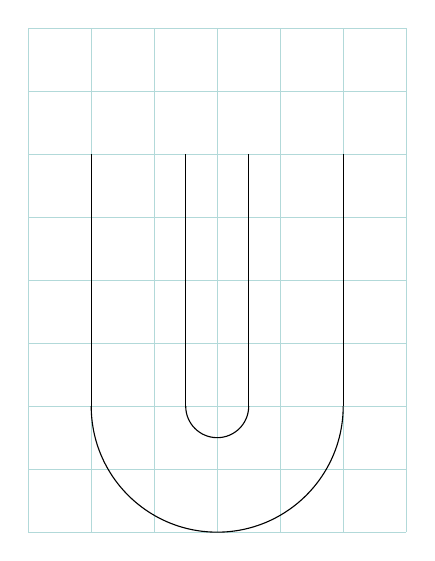
\begin{tikzpicture}[scale=0.8]
\draw[help lines](-3,0) grid(3,8);
\draw(2,2) arc [start angle=0, end angle=-180, radius=2];
\draw(0.5,2) arc [start angle=0, end angle=-180, radius=0.5];
\draw(-0.5,2)--(-0.5,6)(0.5,2)--(0.5,6)(-2,2)--(-2,6)(2,2)--(2,6);



\end{tikzpicture}



%-------------- nomor 13 ---------
\item Dua vektor gaya masing-masing 3 newton dan 4 newton. Jika kedua vektro tersebut saling tegak lurus, maka resultan kedua vektor tersebut adalah . . . .
\pilgan{
\item 3 newton
\item 4 newton
\item [\kunci{C.}] 5 newton
\item 6 newton
\item 7 newton
}

%------------------- nomor 14 -------
\item Dua buah vektor gaya $F_1$ dan $F_2$ bertitik tangkap di 0 seperti pada gambar di bawah ini. Resultan kedua vektor pada sumbu $x$ dan $y$ berturut-turut adalah . . .

\pilgan{
\item $30\sqrt{3}$ N dan 30 N
\item $30\sqrt{3}$ N dan 10 N
\item $30$ N dan $30\sqrt{3}$ N
\item [\kunci{D.}] 10 N dan $30\sqrt{3}$ N
\item 10 N dan $10\sqrt{3}$ N
}

%----------------- nomor 15 ------------
\item Berapa resultan dari ketiga vektor di bawah ini . . . .


\pilgan{
\item 125 N
\item 100 N
\item 75 N
\item [\kunci{D}.]50 N
\item 25 N
}


%-------------- nomor 16 --------------
\item Resultan ketiga vektor pada gambar berikut adalah . . . 

\pilgan{
\item 20 N
\item 15$\sqrt{2}$ N
\item 10 N
\item 10$\sqrt{2}$ N
\item [\kunci{E.}] 5$\sqrt{2}$ N
}

%-------------- nomor 17 ----------------
\item Berapakah besarnya resultan dari kedua gaya di bawah (dalam N) . . .
\pilgan{
\item $5\sqrt{19}$
\item $4\sqrt{19}$
\item $3\sqrt{19}$
\item $2\sqrt{19}$
\item $1\sqrt{19}$
}

%------------- nomor 18 ----------------
\item Dua buah vektor $F_1$ dan $F_2$ bertitik tangkap sama membentuk sudut 90$^o$. Resultan kedua vektor membentuk sudut 60$^o$ terhadap vektor $F_1$. Apabila vektor $F_1$ = 40 N maka vektor $F_2$ = . . . .
\pilgan{
\item $20\sqrt{3}$ N
\item $40\sqrt{3}$ N
\item $60\sqrt{3}$ N
\item $80\sqrt{3}$ N
\item $100\sqrt{3}$ N
}

%--------------- nomor 19 -------------
\item Gatot berjalan ke arah barat sejauh 50 m, kemudian berbelok ke arah utara 10 m, lalu berbelok ke arah timur 10 m dan diakhiri dengan berbelok ke utara sejauh 20 m. Besar perpindahan yang dilakukan Gatot adalah  . . 
\pilgan{
\item 40 m
\item 45 m
\item [\kunci{C.}]50 m
\item 55 m
\item 60 m
}
\hide{
Untuk mengerjakan soal seperti ini, pertama-tama digambar dahulu perpindahan gatot

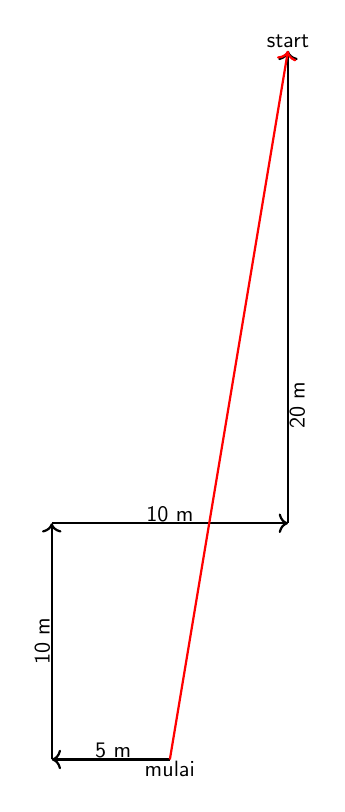
\begin{tikzpicture}[scale=0.6]
\draw[thick,->](0,0)--(-2.5,0);
\draw[thick,->](-2.5,0)--(-2.5,5);
\draw[thick, ->](-2.5,5)--(2.5,5);
\draw[thick,->](2.5,5)--(2.5,15);
\node at (-1.2,0.2)[scale=0.8]{5 m};
\node at (-2.7,2.5)[scale=0.8,rotate=90]{10 m};
\node at (0,5.2)[scale=0.8]{10 m};
\node at (2.7,7.5) [scale=0.8,rotate=90]{20 m};
\node at (0,-0.2) [scale=0.8]{mulai};
\node at (2.5,15.2) [scale=0.8]{start};
\draw[red,thick,->](0,0)--(2.5,15);
%\draw[blue,->]
\end{tikzpicture}
\begin{tabular}{cccc}
\hline
 & $x$ & $y$ &\\ \hline
$r_1$ & -50 m & 0& \\ \hline
$r_2$ & 0 &10 m& \\ \hline
$r_3$ & 10 m & 0 &  \\ \hline
$r_4$ & 0  & 20 m  & + \\ \hline
$\Sigma$ & -40 m & 30 m & \\ \hline
\end{tabular}
\vspace{1cm};
$$ R = \sqrt{x^2+y^2}=\sqrt{(-40)^2+(30)^2}=50 \text { m}$$
}

%------------ nomor 20 ---------------
\item Seorang petugas pos mengendarai sebuah truk pengirim barang dengan rute seperti sebagai berikut. Pertama dia berjalan ke barat sejauh 5 km, kemudian berbelok ke selatan sejauh 2 km dan berbelok 37$^o$ ke barat sejauh 5 km. Jika $\cos 53^o$ = 0,6 maka besar perpindahan truk tersebut adalah . . . 
\pilgan{
\item [\kunci{A.}]10 km
\item 8 km
\item 6 km
\item 4 km
\item 2 km
}
\hide{
Untuk mengerjakan soal seperti ini, pertama digambar dulu perpindahan petugas pos tersebut
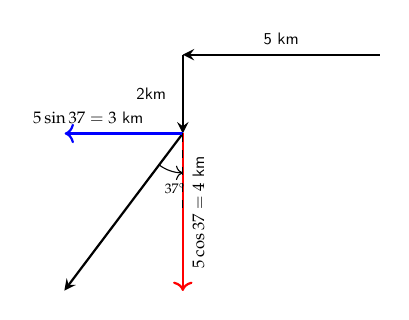
\begin{tikzpicture}
\draw[thick,-stealth](0,0)--(-2.5,0);
\draw[thick,-stealth](-2.5,0)--++(0,-1);
\coordinate (a) at (-2.5,-3);
\coordinate (o) at (-2.5,-1);
\coordinate (b) at ($(-2.5,-1)+(233:2.5)$);
\draw[thick,-stealth](-2.5,-1)--++(233:2.5);
\pic [draw, ->, "", angle radius=0.5 cm, angle eccentricity=1.2]{angle=b--o--a};
\draw[thick, ->,red](-2.5,-1)--(-2.5,-3);
\draw[thick, ->, blue](-2.5,-1)--(-4,-1);

\node at (-2.6,-1.7) [scale=0.5]{$37^\circ$};
\draw[dashed](-2.5,-1)--(-2.5,-2);
\node at (-1.25,0.2)[scale=0.6]{5 km};
\node at (-2.9,-0.5)[scale=0.6]{2km};
\node at (-3.7,-0.8) [scale=0.6]{$ 5 \sin 37 = 3 \text{ km}$};
\node at (-2.3, -2) [scale=0.6, rotate=90]{$ 5 \cos 37= 4 \text{ km}$};
\end{tikzpicture}

Untuk menghitung jumlah perpindahannya dijumlah komponen perpindahan ke arah $x$ dan ke arah $y$
\begin{tabular}{cccc}
\hline
 & $x$ & $y$ &\\ \hline
$r_1$ & -5 km & 0& \\ \hline
$r_2$ & 0 & -2 km& \\ \hline
$r_3$ & -3 km & -4 km & + \\ \hline
$\Sigma$ & -8 km & -6 km & \\ \hline
\end{tabular}
\vspace{1cm};
$$ R = \sqrt{x^2+y^2}=\sqrt{(-8)^2+(-6)^2}=10 \text { km}$$
}
\end{enumerate}
\end{multicols*}
\end{document}

%--------------------- Selesai-------
